\documentclass{beamer}
\usepackage[utf8]{inputenc}
\usepackage{amsmath}
\usetheme{metropolis}

\setbeamercolor{block title}{bg=gray!30}
\setbeamercolor{block body}{bg=gray!10}

\title{An introduction to Python}
\author{Thibaut Lunet, Aitor Pérez}

\date{March 19, 2018}

\begin{document}
	\maketitle
	
	\begin{frame}{History}
		XXX slkdjlksj
	\end{frame}

	\begin{frame}{Functioning principles}
		XXX dsdskldj
		
		
		\begin{block}{slkdfjslk}
			kdjfkdjfkdj
		\end{block}
	\end{frame}


	\begin{frame}{MATLAB vs. Python}
		Some drawbacks of MATLAB:
		\begin{itemize}
			\item It is a proprietary software
			\item It does not scale properly to big projects
			\item Hard to work with in a general framework other than numerical computing
			\item Tricky code organization (function name = file name)
			\item Toolboxes are distributed/purchased separately
		\end{itemize}
	
		\vspace{10pt}
	
		Python solves all of these problems!
	\end{frame}

	\begin{frame}{How to get Python}
		We are going to use the \textbf{miniconda} installer, which is cross-platform and provides package management, together with the \textbf{spyder} IDE.
		
		\begin{enumerate}
			\item XXX Thibaut
			\item Peux-tu completer
			\item Cette liste de choses à faire
			\item Pour obtenir miniconda + spyder?
			\item Merci! :D
		\end{enumerate}
	\end{frame}

	\begin{frame}{Practical tools}
		XXX jfdhjfhdf
	\end{frame}

	\begin{frame}{Basic commands}
		\begin{itemize}
			\item Basic arithmetic logic operations: \texttt{+}, \texttt{-}, \texttt{*}, \texttt{/}, \texttt{\%}, \texttt{<}, \texttt{<=}, \texttt{==}, \texttt{!=}, \texttt{and}, \texttt{or}, \texttt{not}, etc.
			\item No need to declare variables
			\item Basic types: \texttt{int}, \texttt{float}, \texttt{double}, \texttt{complex}, \texttt{bool}, \texttt{str}
			\item Container types: \texttt{list}, \texttt{dict}
			\item Tabs matter!
		\end{itemize}
	
		XXX À completer: ajouter exemples (images?) pour chaque point.
		
	\end{frame}

	\begin{frame}{Hello world!}
		XXX Juste un exercice pour voir s'ils ont bien installé python et spyder.
	\end{frame}

	\begin{frame}{Lists}
		Python allows to use list comprehension:
		
		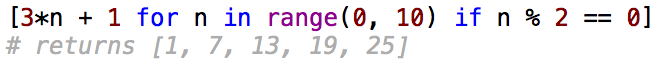
\includegraphics[height=20pt]{img/lists.png}
		
		\vspace{20pt}
		
		\begin{block}{Exercise 1}
			Rewrite the \texttt{filter\_positive} function and reduce it to one line.
		\end{block}
	\end{frame}

	\begin{frame}{File I/O}
		XXX sdjhj
	\end{frame}

	\begin{frame}{Exercise 3 - Numpy?}
		XXX Maybe a small numpy example?
	\end{frame}

\end{document}